\section {Environmental disturbances}
  \label{chap:distTorques}
%
The environmental disturbances can cause a change in the total momentum of the spacecraft. At the following chapter will be accounted the main disturbing torques that are aerodynamic, solar radiation, gravity gradient and magnetic disturbance torque, as well as the $J_{2}$ orbital perturbation due to oblateness of the Earth .
\subsection{Orbit perturbation - $J_2$ }\label{chap: j2}
Due to Earth's spin, its shape is oblate rather than spherical. This non spherical mass distribution of the Earth, affects a satellite motion in LEO. The gravitational potential is corrected using spherical harmonics which depend only on the latitude. These harmonics affect the satellite, determining its orbit difference compared to ideal mathematical models.
An approximation of the gravitational potential of the Earth is \cite{SADC}\cite{PrevPro}:
\begin{flalign}
U \approx -\frac{\mu}{r} \left[1 - \sum_{n=2}^{\infty} \left(\frac{R_e}{r}\right)^{n} J_n P_n cos(\theta)  \right ] = \frac{\mu}{r} [U_0 + U_{J_2} + ...]
\label{eq:Pr341}
\end{flalign}
%\nomenclature[S]{\textbf{$j_2$}}{Zonal harmonic coefficient}
%\nomenclature[S]{\textbf{$R_e$}}{Equatorial radius}
describing deviations of the potential to the south and north direction,
with $P_n$ be Legendre polynomial, $\theta$ be a spherical polar coordinate, $U_0$ = -1, $U_{J_2}$ = $\left(\frac{R_e}{r}\right)^{2} J_2 \frac{1}{2} (3 cos^2 \theta -1) $ and ${J_2 = 1.0826*10^{-3}}$ be a zonal numerical coefficient and the other terms($j_3,j_4,...$) been discarded since are less significant compared to $j_2$. The force caused by the $j_2$ term is obtained as 
\begin{flalign}
\vec F_{j2} = -m \nabla U
\label{eq:Pr3431}
\end{flalign}
%\nomenclature[S]{\textbf{$F_{j2}$}}{Force caused by the $j_2$ effect}
with the vector $\vec F_{j2}$ expand to the force components \cite{SIDI}\cite{PrevPro}  :
\begin{flalign}
F_x = -\frac{\partial U}{\partial x} = \mu \left[ -\frac{x}{r^3} + A_{J_2} \left(15 \frac{xz^2}{r^7} - 3\frac{x}{r^5}   \right ) \right ]       \\
F_y = -\frac{\partial U}{\partial y} = \mu \left[ -\frac{y}{r^3} + A_{J_2} \left(15 \frac{yz^2}{r^7} - 3\frac{y}{r^5}   \right ) \right ]       \\
F_z = - \frac{\partial U}{\partial z} =  \mu \left[ -\frac{z}{r^3} + A_{J_2} \left(15 \frac{z^3}{r^7} - 3\frac{z}{r^5}   \right )  \right]       
\label{eq:Pr34331}
\end{flalign}
where $A_{J_2}  = \frac{1}{2} J_2 R_e^2$ and and $R_e$ is the mean radius o the Earth at the equator
\subsection*{Aerodynamic disturbance torque}\label{chap:disturbances}
%
Gas molecules, in a LEO(low Earth orbit) collide with the surface of the satellite causing
a force which direction opposes the direction of the satellites velocity vector. This Aerodynamic force can be modeled as \cite{SADC,PrevPro}  


\begin{flalign}
	\vec{F_A} = -\frac{1}{2} \rho \ C_D \ A_{\perp}   \vec{v}^2
	\label{eq:ec1c}
\end{flalign}

where $\rho$ is the atmospheric density  
is chosen to be constant and equal to $1.454 \cdot 10^{-13} Kg/{m^3}$ based on the Committee on Space Research\cite{FSA}, $\vec{v}$ is the satellite velocity vector, $A_{\perp}$ is the area perpendicular to the velocity and $C_D$ is the drag coefficient and is chosen to be equal to 1.5 \cite{SADC}\cite{PrevPro} for simulation purposes. If the calculation of the lifetime of the satellite is of great importance a more accurate drag coefficient should be used.

\begin{figure}[h!]
	\centering
	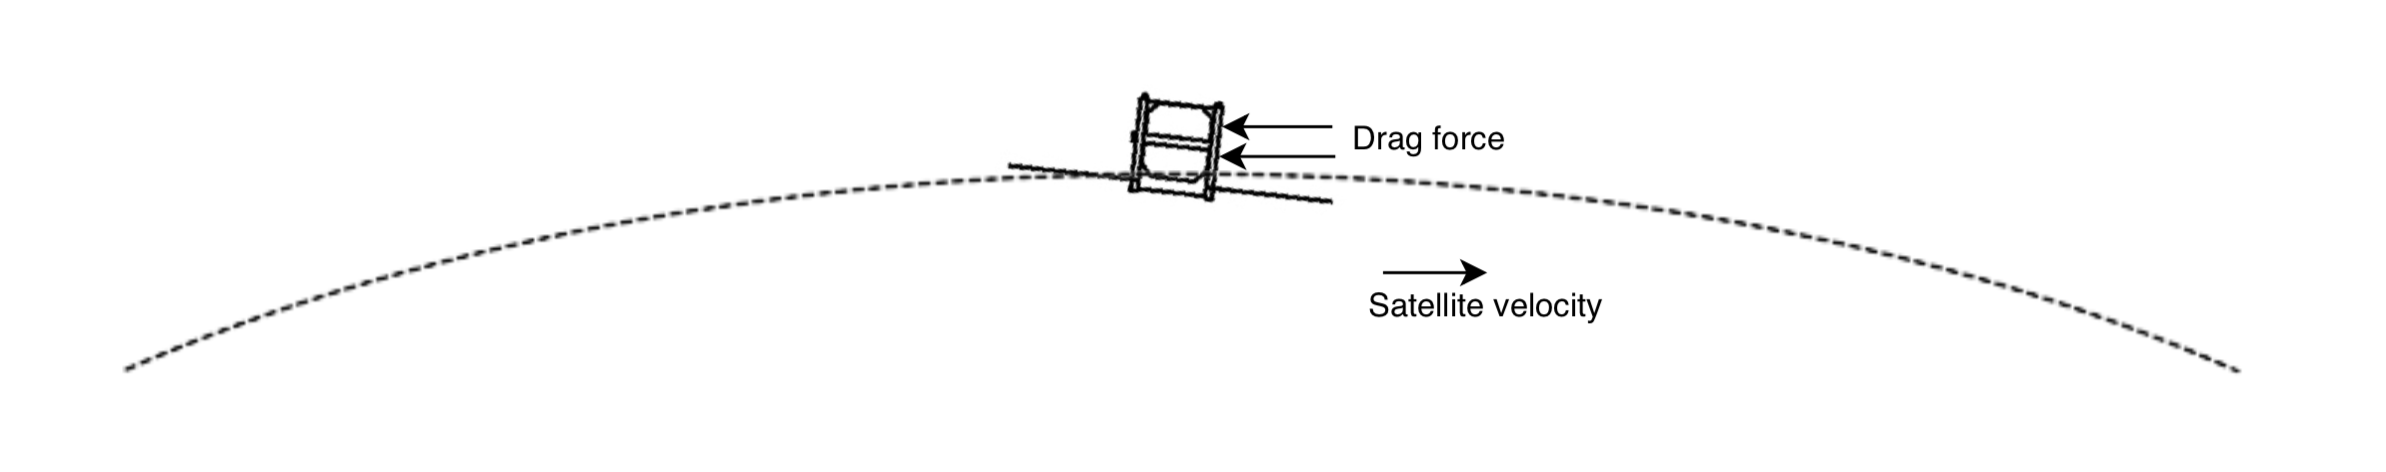
\includegraphics[width=0.9\linewidth]{figures/AFF}
	\caption{Aerodynamic disturbance force action on a orbiting satellite}
	\label{fig:af}
\end{figure}

Using the \eqref{eq:ec1c}, the aerodynamic torque acting on the satellite can be written as 
\begin{flalign}
	\vec N_{drag} = \vec r_{s} \times  \vec F_{A} 
	\label{eq:drag}
\end{flalign}
where:\\
$\vec r_{s}$ is the vector from the centre of mass of the satellite to the geometric centre of the exposed area
%\nomenclature[S]{\textbf{$\vec N_{drag}$}}{Drag disturbance torque}
\subsection*{Solar radiation disturbance torque}\label{chap: disturbances2}

Solar radiation pressure is emitted from various sources such as reflection from the Earth's atmosphere, from solar wind and direct radiation from the sun to the surface of the satellite\cite{SADC}\cite{PrevPro}  . Direct radiation is larger and only this source will be taken into account.
		\begin{figure}[H]
			\centering
			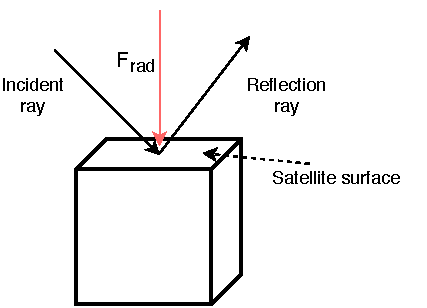
\includegraphics[width=0.5\linewidth]{figures/solar_rad2}
	\caption{ Sun radiation acting on satellite surface}
	\label{fig:radf}
		\end{figure}

The solar flux is given as
\begin{flalign}
	P = \dfrac{F_s}{c}
	\label{eq:flux2}
\end{flalign}

where $F_s$ is the intensity or mean energy flux given as 1358 [$W/m^2$] and $c$ is the speed of light. The solar radiation force $\vec F_{rad}$ can be expressed as 

\begin{flalign}
	\vec {F_{rad}} = C_{a} P A \ \hat{S}
	\label{eq:Pres}
\end{flalign}
where $C_{a}\in [0,2]$ is the absorption coefficient which depends on the material of the satellite with 2 be the value of totally reflected beam and for simulation purposes is chosen to be 1.5, $P$ is the solar flux, $A$ is the radiated surface area, and $\hat{S} =\frac{\vec {r_{sun,sat}}}{||\vec {r_{sun,sat}}||}$ is the unit vector from the satellite to the sun. The solar radiation torque can be computed as 
\begin{flalign}
	\vec N_{rad} = \vec r_{s} \times  \vec F_{rad} 
	\label{eq:solar}
\end{flalign}
where $\vec r_{s}$ is the vector from the center of mass of the satellite to the center of pressure.
%
%\nomenclature[S]{\textbf{$P$}}{Solar flux}
%\nomenclature[S]{\textbf{$\vec {r_{sun,sat}}$}}{vector from the satellite to the sun}
%\nomenclature[S]{\textbf{$C_{a}$}}{Absorption coefficient}
%\nomenclature[S]{\textbf{$F_{rad}$}}{solar radiation force}
%\nomenclature[S]{\textbf{$\vec N_{rad}$}}{Solar radiation torque}
%
\subsection*{Gravity Gradient disturbance torque}\label{chap: disturbances3}
Contrary to $j_{2}$ effect, in order to derive an expression for the gravitational torque exerted about the mass center of the satellite, it is assumed symmetrical and spherical Earth's mass distribution  \cite{SADC}.
The gravity gradient effect about the center of mass of the satellite is a consequence of the non-uniform gravitational field of the Earth. If the gravitational field was uniformly distributed no torque would be present. The force to an infinitesimal element $d\vec{F_{i}}$ to a distance $R_{i}$ from the center of the Earth can be written
%
\begin{flalign}
d\vec F_{i} = \dfrac{-\mu\vec{R_{i}}dm_{i}}{R_{i}^{3}} 
\label{eq:ref9876}
\end{flalign}
as it can be seen in \figref{fig:gg}. The torque about the geometric center of the satellite can be written as 
 %
 \begin{flalign}
 \vec N_{gra}^{i} = r_{i}\times d\vec F_{i}
 \label{eq:ref9876875}
 \end{flalign}
 %
 Assuming that the center of mass is aligned with the geometric center, the torque about the center of mass of the satellite can be expressed as\cite{SADC}\cite{PrevPro}  

%\nomenclature[A]{\textbf{$\vec N_{gra}$}}{Gravity Gradient torque}
\nomenclature[A]{\textbf{COM}}{Center of Mass}
%\nomenclature[S]{\textbf{$d\vec F_{i}$}}{Gravity force to an infinitesimal element}
%
\begin{flalign}
	\vec N_{gg} &= \dfrac{3\mu}{\vec R_{sc}^3}[\vec{\hat R_{sc}} \times(\vec{I} \ \vec{\hat R_{sc}}] 
	\label{eq:ref4}
\end{flalign}
where $\vec{\hat R_{sc}}$ is the unit vector from geometric centre of the earth's to the satellite's geometric centre, $\mu = G*m_{earth}$ with $G$ be the Gravitational constant $6.6740*10^{-11}$ [$m^{3} kg^{-1} s^{-2}$] and $\underline I$ is the inertia matrix of the satellite. 

\begin{figure}[H]
	\centering
	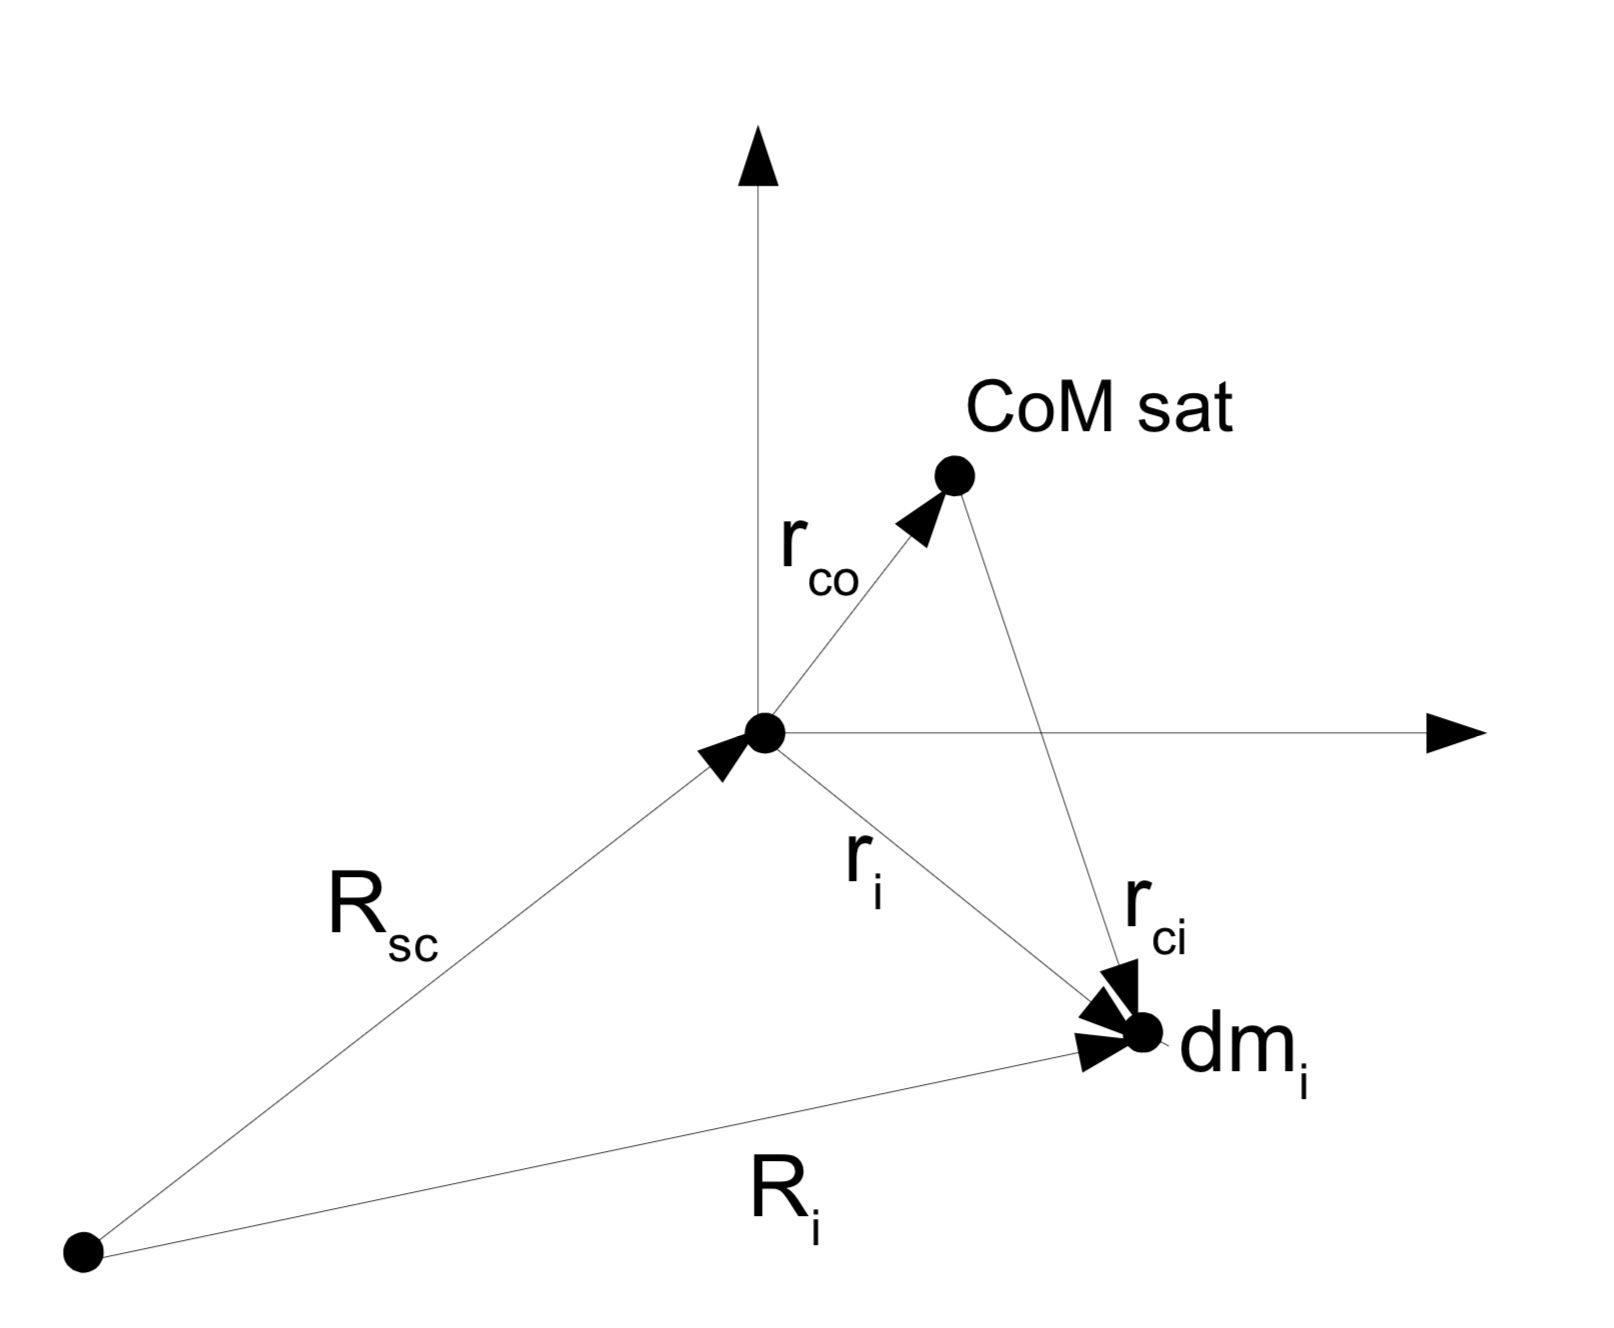
\includegraphics[width=0.5\linewidth]{figures/ggt}
	\caption{Gravity gradient torque computation using the coordinate system}
	\label{fig:gg}
\end{figure}

\subsection{Magnetic residual }
When the satellite orbits the Earth, due to the interference of the magnetic field of the Earth and the satellite magnetic residual, an extra disturbance torque is generated. Because the satellite can not be perfectly isolated, the actuators and sensors will produce a residual magnetic moment. Similarly like magnetorqers, the torque generated by the magnetic residual can be computed using:
\begin{flalign}
\vec N_{mr} = \vec m \times \vec B
\label{eq:st}
\end{flalign}
where $\vec m$ is the magnetic moment and $\vec B$ is the magnetic field of the Earth.

The magnetic field of the Earth can be approximated using \cite{SMAD}:
\begin{flalign}
B = \dfrac{2M}{R^3}
\label{eq:ftf}
\end{flalign}
where $M$ is the Earth magnetic moment and $R$ is the distance from the Earth to the center of the satellite.

%\nomenclature[SNmr]{$\vec N_{mr}$}{The torque generated by the magnetic residual }
%\nomenclature[Smr]{$\vec m_{mr}$}{The magnetic residual}
%\nomenclature[SB]{$\vec B$}{The magnetic field of the Earth}
%\nomenclature[SM]{$\vec M$}{The Earth magnetic moment }
%\nomenclature[SR]{$\vec R$}{The distance from the Earth to the center of the satellite}

\subsection{Total disturbance torque}
The total disturbance torque that the satellite is subject to is presented as follows:

\begin{flalign}
	N_{dist} = N_{drag} + N_{rad} + N_{gg} + N_{mr}
	\label{eq:TDT}
\end{flalign}

The magnitude of the torque is computed in MATLAB using the AAUStudentSpace toolbox and gather in the following table:
\begin{table}[H]
	\centering
	\label{TTdist}
	\begin{tabular}{|l|c|l|}
		\hline
		\textit{\textbf{Disturbance}} & \textit{\textbf{\begin{tabular}[c]{@{}c@{}}Torquet magnitude at a given\\  moment in the orbit (nNm)\end{tabular}}} & \multicolumn{1}{c|}{\textit{\textbf{\begin{tabular}[c]{@{}c@{}}Torque \\ magnitude (Nm)\end{tabular}}}} \\ \hline
		\textit{Aerodynamic}          & 1.52                                                                                                                &                                                                                                         \\ \hline
		\textit{Gravitaional}         & 0.86                                                                                                                &                                                                                                         \\ \hline
		\textit{Radiation}            & 1.25                                                                                                                &                                                                                                         \\ \hline
		\textit{Magnetic residual}    & 48                                                                                                                  &                                                                                                         \\ \hline
	\end{tabular}
	\caption{Environmental disturbance torques}
\end{table}
%Total torque magnitude is illustrated in figure \ref{fig:totalN}, where the most significant disturbance torque is the magnetic residual.
%\begin{figure}[h!]
%	\centering 
%	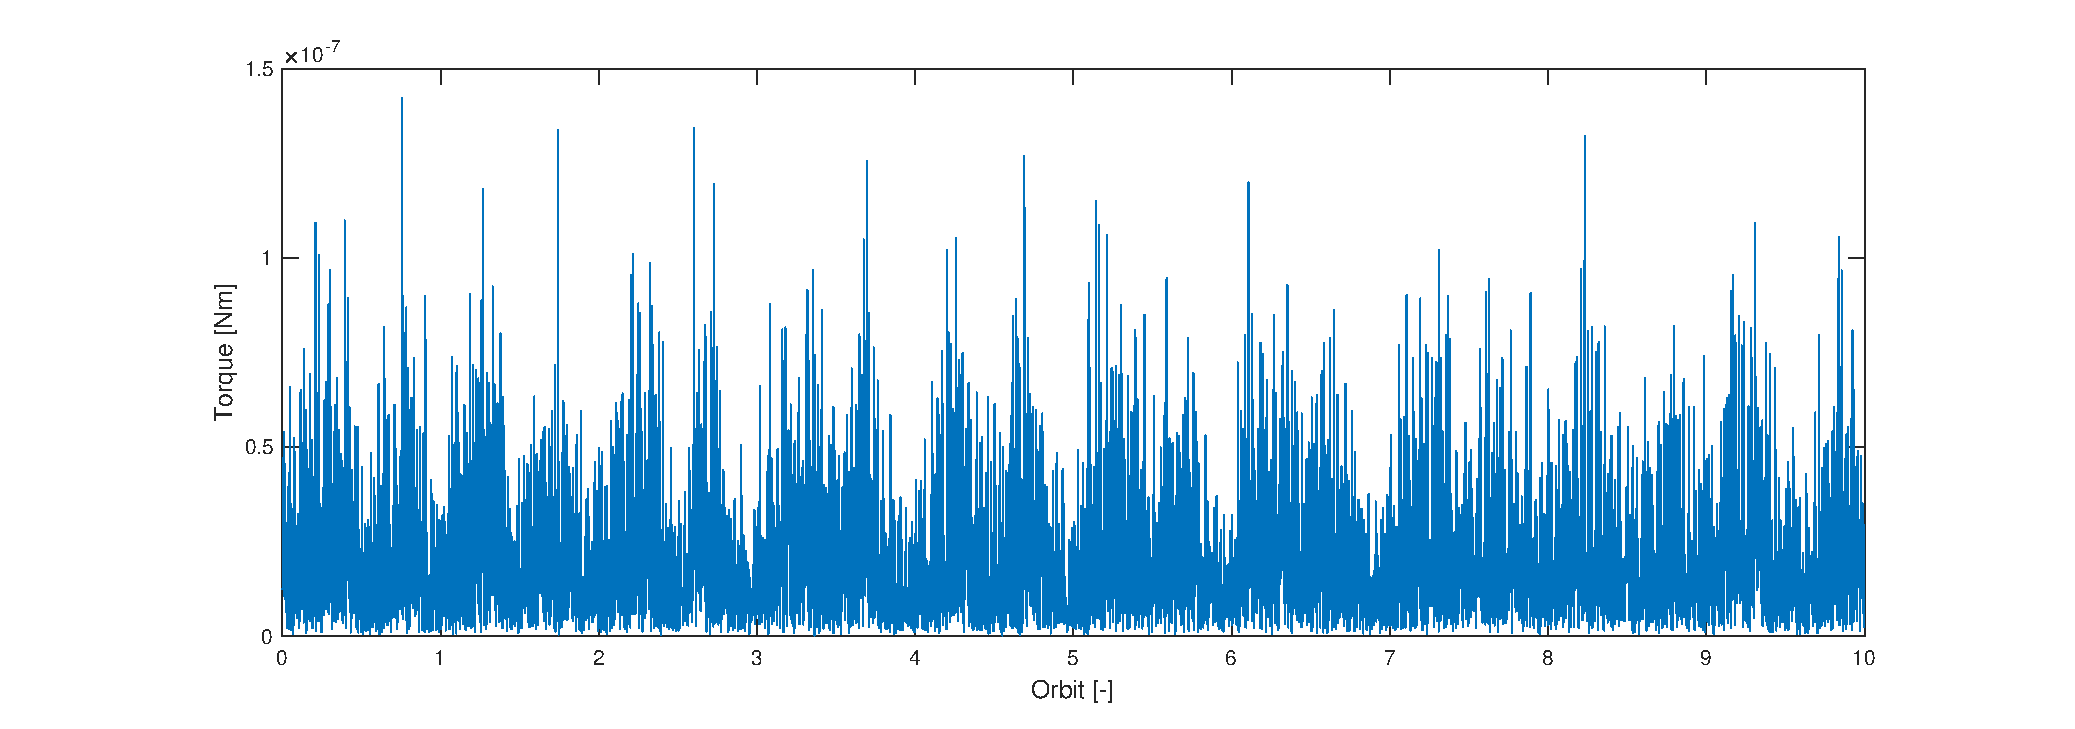
\includegraphics[width=160mm]{figures/total_torque}	
%	\caption{Total torque magnitude}
%	\label{fig:totalN}
%\end{figure}